\subsection{Application of Hidden Markov Model}

The Hidden Markov models were used to analyse the movements. Therefore the process of analsysing is split into two parts. The first part is the training phase, were a new hidden markov model with help of the K-Means algorithm (see  \textcolor{red}{\textbf{ ADD SECTION NUMBER !!!!!}} Application K-Means) is created for the choosen exercise. To get an good hidden markov model from the training phase 10 - 20 repetitions of the exercise are needed. After the Hidden Markov Model was created, each repetition was put into the models and the resulted state sequence was stored for comparing. For the number of state five was a good choice, because less states would cause wrong results and more, would consume too much memory from the smartphone. In the second phase the real analysis of the movements takes place. In this phase the collected three dimensional movement data (acceleration * positional) is put into the Hidden Markov Model and the resulting state sequence is used to calculate how well an exercise was done (see \textcolor{red}{\textbf{ ADD SECTION NUMBER !!!!!}} Filtering).
\begin{figure}[htp]
\centering
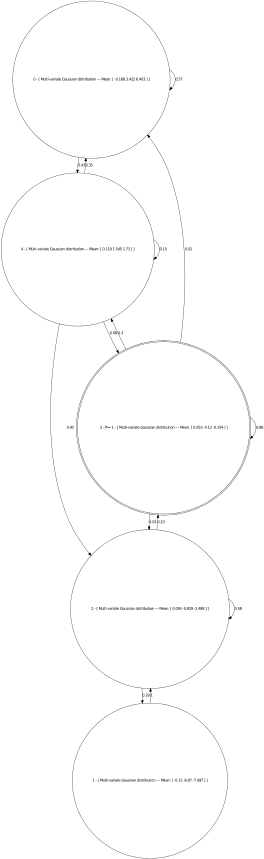
\includegraphics[scale=1.00]{00_resources/figures/output.png}
\caption{Hidden Markov Model}
\label{}
\end{figure}
